\documentclass{article}
\linespread{1.3}
\usepackage[margin=50pt]{geometry}
\usepackage{amsmath, amsthm, amssymb, amsthm, tikz, fancyhdr, float, graphicx, spverbatim, systeme}
\pagestyle{fancy}
\renewcommand{\headrulewidth}{0pt}
\newcommand{\changefont}{\fontsize{15}{15}\selectfont}

\fancypagestyle{firstpageheader}{
  \fancyhead[R]{
    \changefont
    \parbox[t]{4cm}{ % Adjust width as needed
      Michael Huang\\
      EN.625.633.81\\
      Homework 7
    }
  }
}

\begin{document}

\thispagestyle{firstpageheader}
{\Large 

\section*{1.}

\begin{figure}[H]
    \centering
    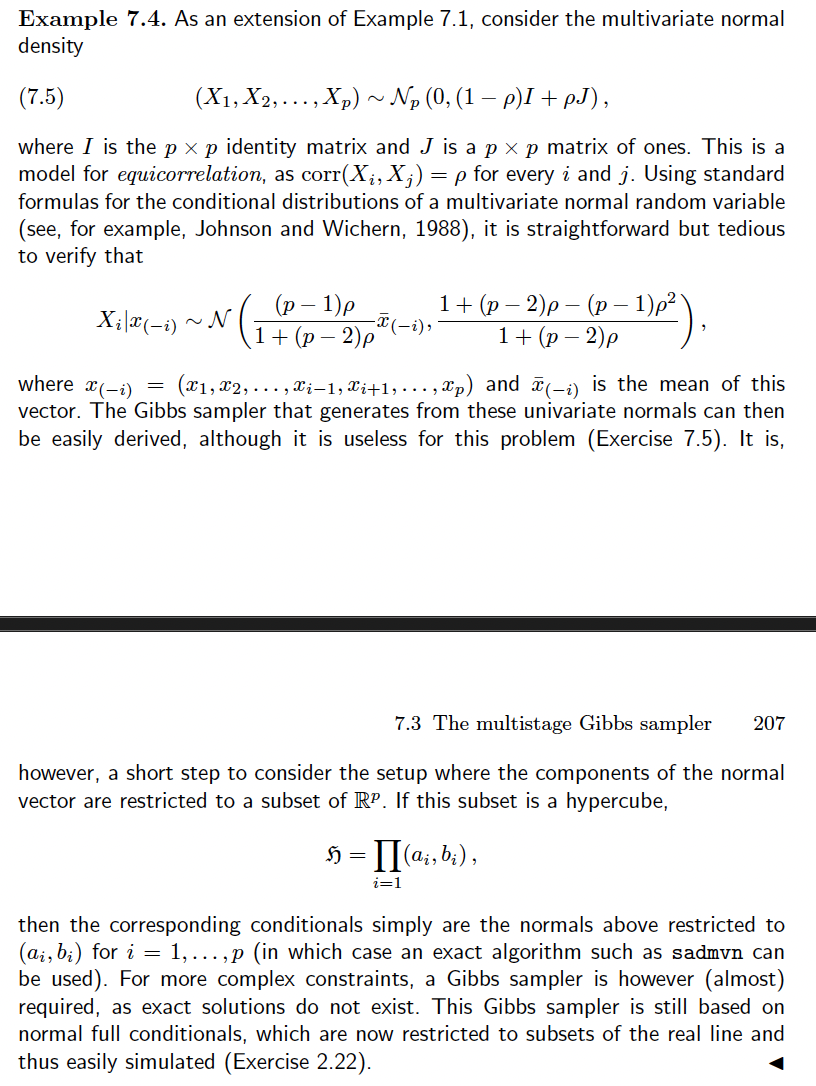
\includegraphics[width=0.75\textwidth]{Example7.4.png}
\end{figure}

\begin{figure}[H]
    \centering
    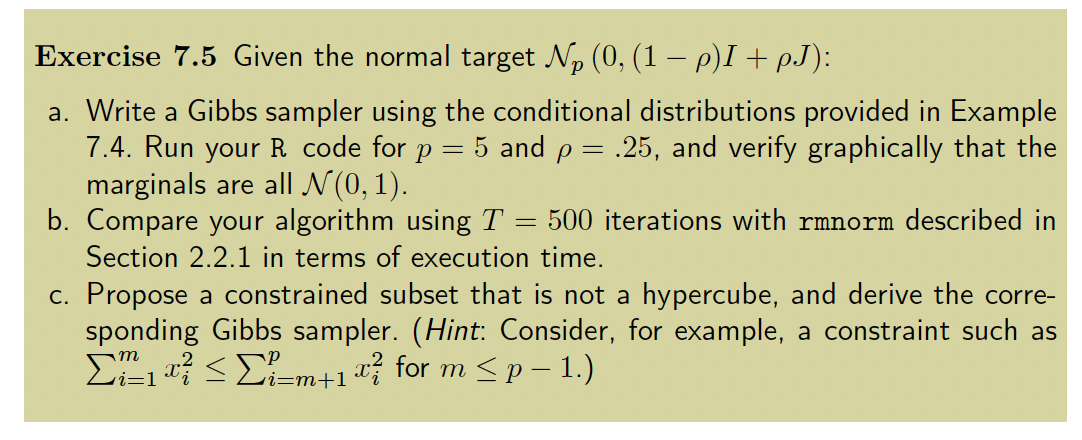
\includegraphics[width=0.75\textwidth]{Exercise7.5.png}
\end{figure}

\subsection*{(a)} 

We are given the target distribution \(X \sim N_p(0, (1 - \rho)I + \rho J)\). From Example 7.4, the conditional distribution of \(X_i\) given all other components is said to be 
\[
  X_i | x_{(-i)} \sim 
  N(\frac{(p - 1) \rho}{1 + (p - 2) \rho}\bar{x}_{(-i)},
  \frac{1 + (p - 2)\rho - (p - 1)\rho^2}{1 + (p-2)\rho})
\]
which we'll use in the code below, following the algorithm of drawing conditionally based on previously drawn values.
\begin{spverbatim}
> # 1. (a)
> n = 500
> p = 5
> rho = 0.25
> gibbs_sample = function(n, p, rho) {
+   # Precomputed constants for conditional distribution from Example 7.4
+   conditional_mean_coeff = ((p - 1) * rho) / (1 + ((p - 2) * rho))
+   sigma_squared = (1 + ((p - 2) * rho) - ((p - 1) * rho^2)) / (1 + ((p - 2) * rho))
+   sigma = sqrt(sigma_squared)
+   
+   X <- array(0, dim = c(n, p)) # init arrays
+   X[1, ] <- rnorm(p) # init chains
+   
+   for (t in 2:n) {
+     x = X[t - 1, ]
+     for (i in 1:p) {
+       x_mean_minus = (sum(x) - x[i]) / (p - 1)
+       x[i] = rnorm(1, mean = conditional_mean_coeff * x_mean_minus, sd = sigma)
+     }
+     X[t, ] = x
+   }
+   
+   X
+ }
> X = gibbs_sample(n, p, rho)
> hist(X[, p], breaks = 50, probability = TRUE,
+      main = paste("Marginals of X with p =", p, ", n =", n))
> curve(dnorm(x, 0, 1), add = TRUE, col = "red")
\end{spverbatim}
\begin{figure}[H]
    \centering
    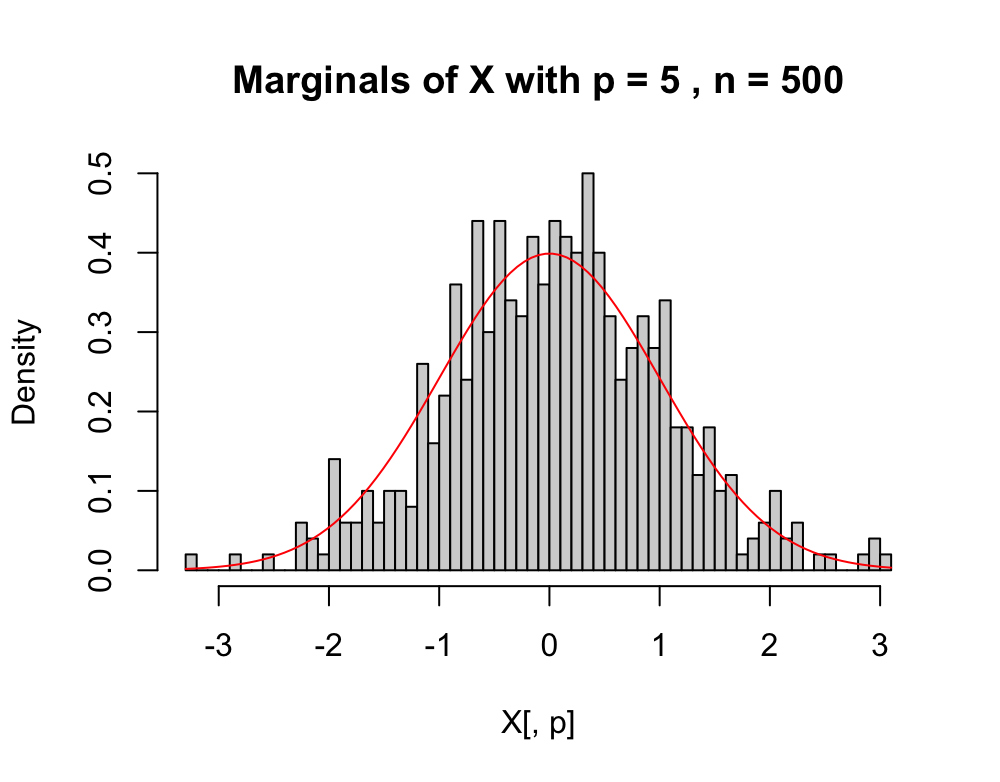
\includegraphics[width=1\textwidth]{1a_hist_comp.png}
\end{figure}
Looking at the graph, it follows \(N(0, 1)\) pretty well.

\subsection*{(b)}

\begin{spverbatim}
> # 1. (b)
> 
> library(mnormt)
> 
> norm_sample = function(n, p, rho) {
+   # sigma as given in Exercise 7.5
+   I = diag(p)
+   J = matrix(1, p, p)
+   sigma = ((1 - rho) * I + rho * J)
+   
+   rmnorm(n, mean = rep(0, p), varcov = sigma)
+ }
> 
> system.time(gibbs_sample(n, p, rho))
   user  system elapsed 
  0.003   0.000   0.002 
> system.time(norm_sample(n, p, rho))
   user  system elapsed 
  0.000   0.000   0.001 
\end{spverbatim}
The rmnorm function seems to be much faster than the Gibbs sampling algorithm, althought this might not be as big of a difference at low iteration count.

}
{\Large 

\section*{2.}

We aim to prove that
\[ 
  f(x, y) = \frac{f(y | x)}{\int \frac{f(y |x)}{f(x | y)} dy} 
\]
Let's start from the right-hand side and start evaluating from there:
\begin{align*}
  &= \frac{f(y | x)}{\int \frac{f(y |x)}{f(x | y)} dy} && \text{Given} \\
  &= \frac{f(y | x)}{\int \frac{f(y |x)}{\frac{f(x,y)}{f(y)}} dy} && \text{Bayes' theorem} \\
  & = \frac{f(y | x)}{\int \frac{f(y |x) \cdot f(y)}{f(x,y)} dy} && \text{Arithmetic} \\
  &= \frac{f(y | x)}{\int \frac{f(y | x) \cdot f(y)}{f(y | x) \cdot f(x)} dy} && \text{Definition of conditional probability} \\
  &= \frac{f(y | x)}{\int \frac{f(y)}{f(x)} dy} && \text{Arithmetic} \\
  &= \frac{f(y | x)}{\frac{1}{f(x)}} && \text{Integration} \\
  &= f(y | x) \cdot f(x) && \text{Arithmetic} \\
  &= f(x, y) && \text{Definition of conditional probability} \\
\end{align*}
Exactly as we sought to prove.

}

\end{document}